\documentclass[]{article}
\usepackage{lmodern}
\usepackage{amssymb,amsmath}
\usepackage{ifxetex,ifluatex}
\usepackage{fixltx2e} % provides \textsubscript
\ifnum 0\ifxetex 1\fi\ifluatex 1\fi=0 % if pdftex
  \usepackage[T1]{fontenc}
  \usepackage[utf8]{inputenc}
\else % if luatex or xelatex
  \ifxetex
    \usepackage{mathspec}
  \else
    \usepackage{fontspec}
  \fi
  \defaultfontfeatures{Ligatures=TeX,Scale=MatchLowercase}
\fi
% use upquote if available, for straight quotes in verbatim environments
\IfFileExists{upquote.sty}{\usepackage{upquote}}{}
% use microtype if available
\IfFileExists{microtype.sty}{%
\usepackage[]{microtype}
\UseMicrotypeSet[protrusion]{basicmath} % disable protrusion for tt fonts
}{}
\PassOptionsToPackage{hyphens}{url} % url is loaded by hyperref
\usepackage[unicode=true]{hyperref}
\hypersetup{
            pdftitle={Appendices},
            pdfborder={0 0 0},
            breaklinks=true}
\urlstyle{same}  % don't use monospace font for urls
\usepackage[margin=1in]{geometry}
\usepackage{graphicx,grffile}
\makeatletter
\def\maxwidth{\ifdim\Gin@nat@width>\linewidth\linewidth\else\Gin@nat@width\fi}
\def\maxheight{\ifdim\Gin@nat@height>\textheight\textheight\else\Gin@nat@height\fi}
\makeatother
% Scale images if necessary, so that they will not overflow the page
% margins by default, and it is still possible to overwrite the defaults
% using explicit options in \includegraphics[width, height, ...]{}
\setkeys{Gin}{width=\maxwidth,height=\maxheight,keepaspectratio}
\IfFileExists{parskip.sty}{%
\usepackage{parskip}
}{% else
\setlength{\parindent}{0pt}
\setlength{\parskip}{6pt plus 2pt minus 1pt}
}
\setlength{\emergencystretch}{3em}  % prevent overfull lines
\providecommand{\tightlist}{%
  \setlength{\itemsep}{0pt}\setlength{\parskip}{0pt}}
\setcounter{secnumdepth}{0}
% Redefines (sub)paragraphs to behave more like sections
\ifx\paragraph\undefined\else
\let\oldparagraph\paragraph
\renewcommand{\paragraph}[1]{\oldparagraph{#1}\mbox{}}
\fi
\ifx\subparagraph\undefined\else
\let\oldsubparagraph\subparagraph
\renewcommand{\subparagraph}[1]{\oldsubparagraph{#1}\mbox{}}
\fi

% set default figure placement to htbp
\makeatletter
\def\fps@figure{htbp}
\makeatother

\usepackage{float} \floatplacement{figure}{H}

\title{Appendices}
\author{}
\date{\vspace{-2.5em}}

\begin{document}
\maketitle

\subsection{Appendix 1: Additional Description of Study
Reaches}\label{appendix-1-additional-description-of-study-reaches}

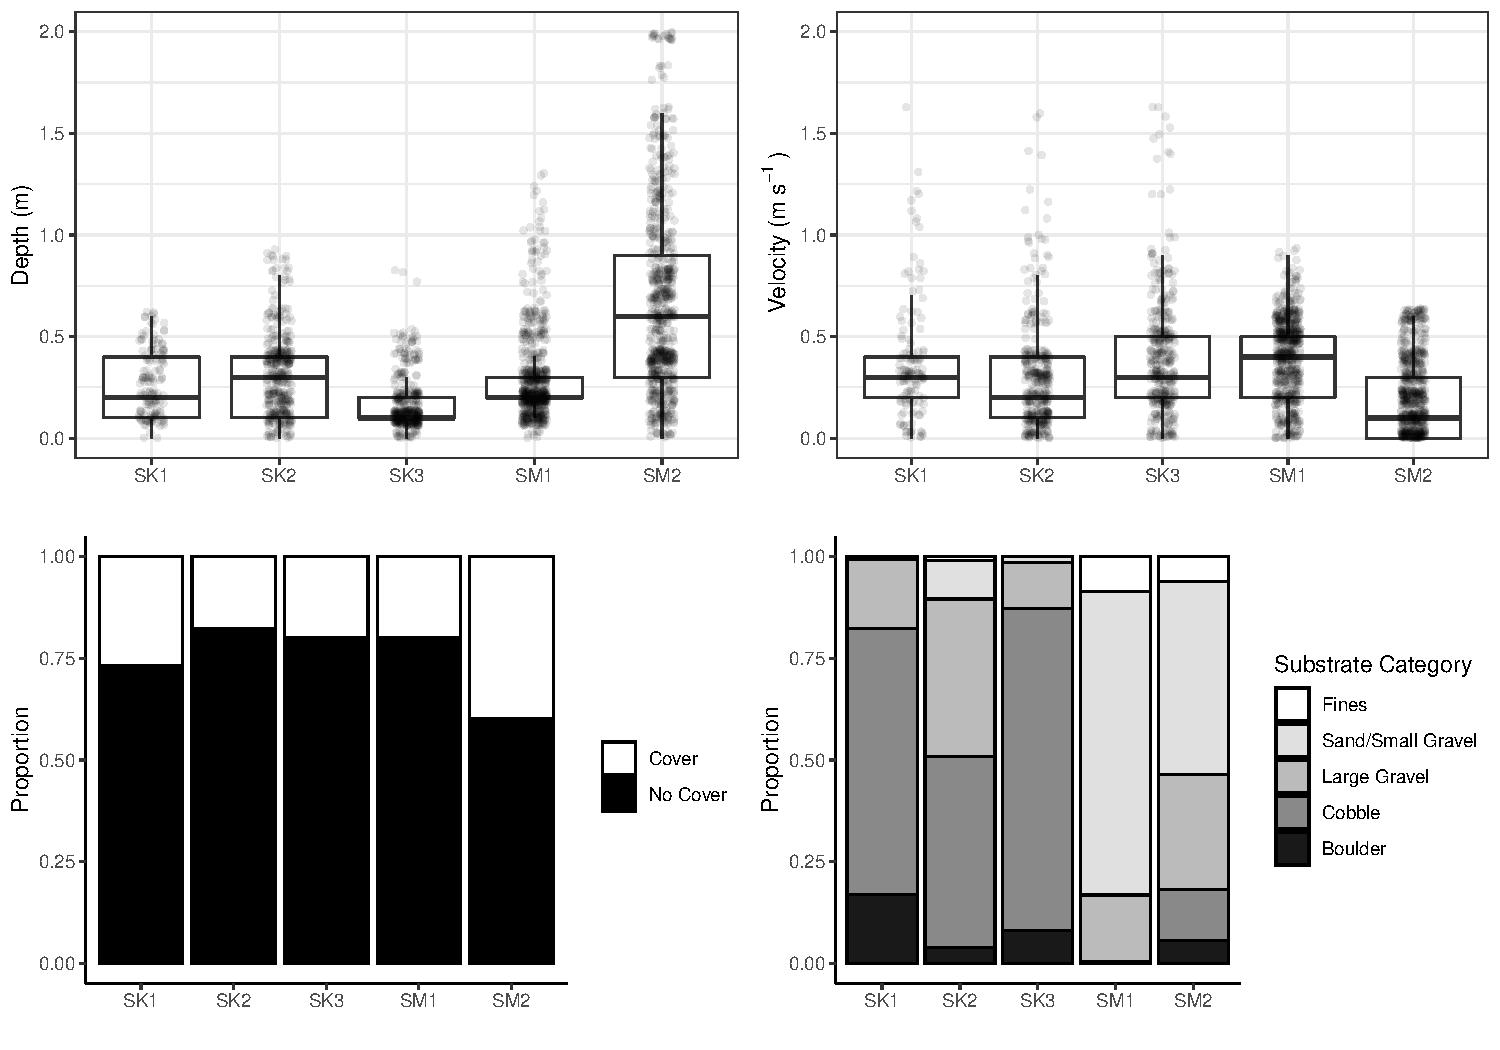
\includegraphics{Final_figures/Appendix_S1}

\textbf{Figure S1} Distributions of habitat conditions measured on
transects at the five study reaches in the mainstem Skagit and the
Summalo. Site locations (Latitude and Longitude in decimal degrees) are
as follows: SK1 (49.208 N., 121.08 W.), SK2 (49.206 N., 121.08 W.), SK3
(49.207 N., 121.07 W.), SM1 (49.264 N., 121.209 W.), and SM2 (49.238 N.,
121.134 W.).

\clearpage

\section{Appendix 2: Additional Details on Cover Addition
Experiment}\label{appendix-2-additional-details-on-cover-addition-experiment}

\emph{Cover box hydraulics}

To account for the potential role of altered hydraulic conditions due to
the addition of cover, we measured velocity in each location before the
cover boxes were installed and four days later following observations of
fish presence. We also estimated velocity at the exact locations of each
foraging fish and noted whether fish appeared to be exploiting
micro-velocity gradients that may have been introduced by the structural
cover associated with the cover box.

To infer whether cover box additions modified hydraulics, we compared
velocity measurements before cover boxes were installed and after they
were retrieved. The six velocity measurement locations were evenly
spaced across a 30 x 15 cm grid. At each location, we measured velocity
at the stream bottom and at 60\% of the water depth. These comparisons
revealed some effects of cover additions on hydraulics. Most notably,
point velocities were reduced in boxes placed in the highest velocity
areas (Figure B1). However, all of the boxes with larger effects on
velocities were predicted to have negative NREI and none were ultimately
colonized by fish.

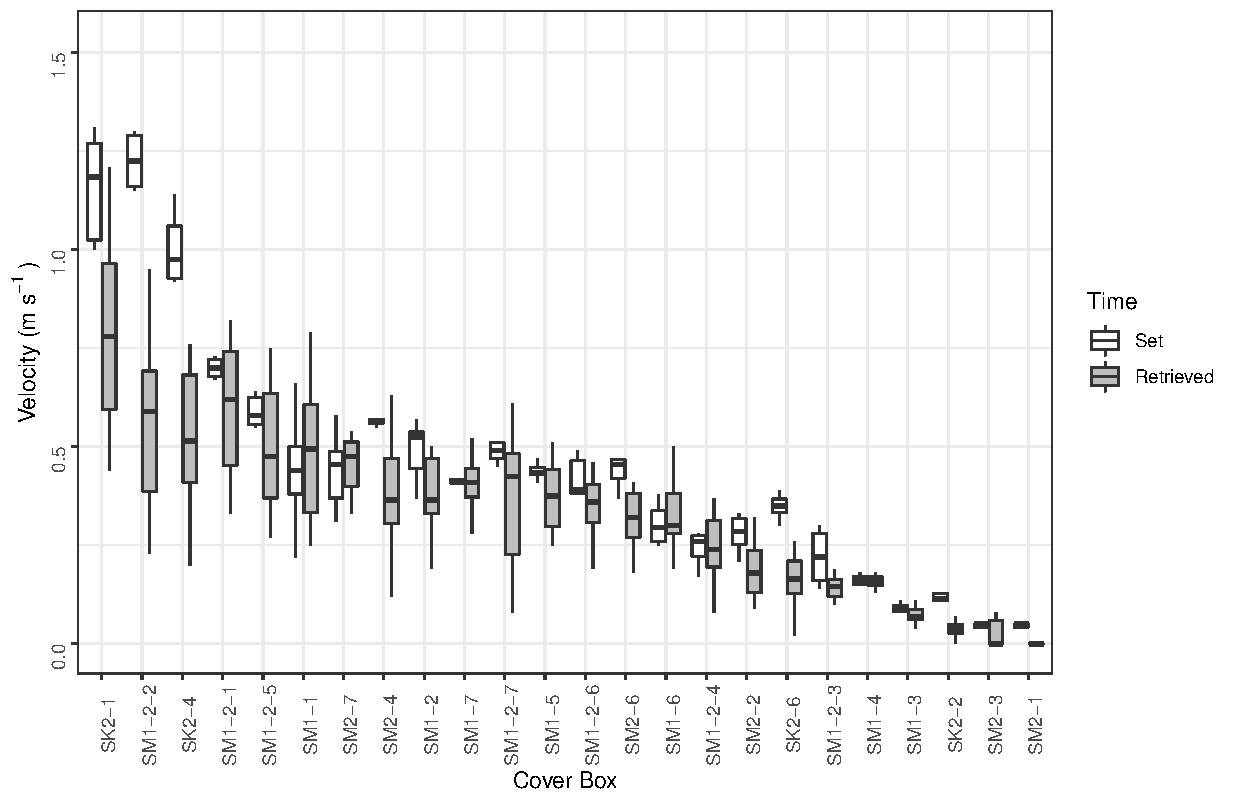
\includegraphics{Final_figures/Appendix_S2}

\textbf{Figure S2} Velocity measurements at each cover box (ordered from
highest to lowest mean velocity) taken before (white) and after (grey)
installation. Boxes represent the 25\% and 75\% quartile ranges and
lines represent the median values.

\clearpage

\emph{Fish Size Distributions}

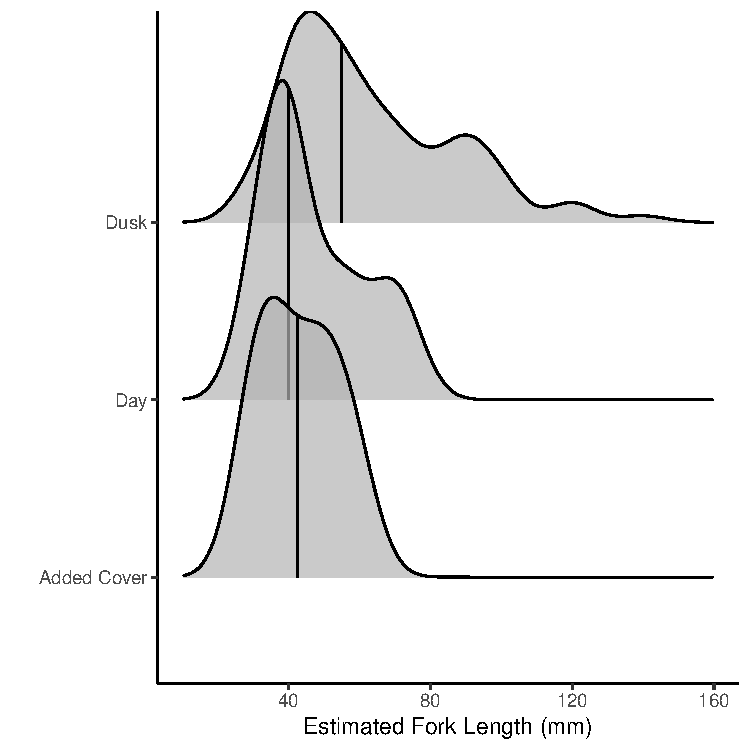
\includegraphics{Final_figures/Appendix_S3}

\textbf{Figure S3} the estimated relative size distributions of rainbow
trout observed foraging under the experimentally added cover compared to
size distributions of fish observed foraging at dusk and during the day.

\emph{Net Rate of Energy Intake Modelling}

We used the free program BioenergeticHSC to implement the NREI model.
Details of how the program works can be found at
(\url{http://www.aferu.ca/rosenfeld-lab-bioenergetichsc}). We estimating
NREI using the average velocity measured from each cover box and a
constant depth of 20 cm (the height of the box). We averaged all daytime
drift measurements for this analysis and used a standard fish length of
4.5 cm (approximating the averaged daytime forager). Mass was estimated
using a length-mass relationship for each species developed from Silver
Hope Creek, an adjacent watershed where we had previously conducted
electrofishing surveys (Naman et al. 2019).

We assumed fish held focal points at 80\% of the water depth, which was
consistant with empirical observations. We also assumed a logarithmic
vertical velocity profile, with a bed roughness height of 2 cm.
Temperature was set at 10°C. Other options were set as following: the
rainbow trout swimming cost submodel; the rainbow trout Wisconsin
bioenergetics option for energy assimilation; turbitity set to 0; prey
detection and reaction distance multipliers set to 1; diet optimization
on; and a spatial grid resolution of 2 cm.

\clearpage

\section{Appendix 3: Invertebrate drift
results}\label{appendix-3-invertebrate-drift-results}

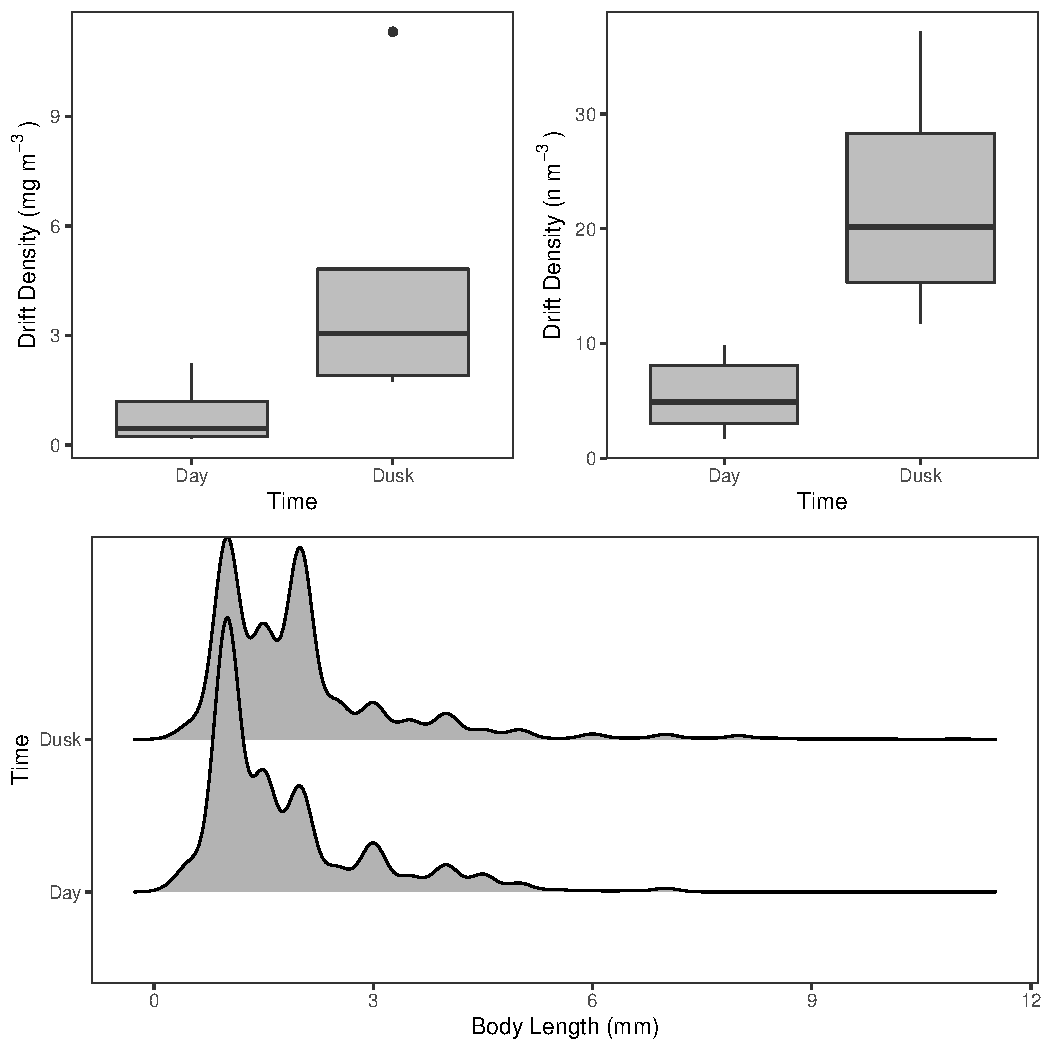
\includegraphics{./Final_figures/Appendix_S4.pdf}

\textbf{Figure S4} Top: concentration of invertebrate drift (mg
m\(^{-3}\) and number m\(^{-3}\)) measured during the day and at dusk.
Bottom: Relative distributions of individual drifting invertebrate body
size (mm) during the day and at dusk.

\section*{References}\label{references}
\addcontentsline{toc}{section}{References}

\hypertarget{refs}{}
\hypertarget{ref-Naman2019}{}
Naman, Sean M., Jordan S. Rosenfeld, Jason R. Neuswanger, Eva C. Enders,
and Brett C. Eaton. 2019. ``Comparing correlative and
bioenergetics‐based habitat suitability models for drift‐feeding
fishes.'' \emph{Freshwater Biology} 64 (9): 1613--26.
doi:\href{https://doi.org/10.1111/fwb.13358}{10.1111/fwb.13358}.

\end{document}
